\chapter{视频编码概述}
\label{cha:coding}

\section{VP9视频编码标准}
\label{sec:vp9}

% \subsection{HEVC与H.265}

\subsection{基本编码单元:块}
\label{sec:block}

视频流可以看成由许多图片按顺序播放组成,而这些“图片”正是视频流的基本单位:帧。尽管视频流以帧为
基本单位,但在视频分辨率日益增长的今天,帧作为视频编码的基本单位过于庞大了。以3840x2160
像素的典型4K视频为例,稍加计算我们不难发现,一帧中包含着多达 $3840x2160 = 8294400$ 像素点,
以800万以上的像素点作为基本单位,对于后续的分割、预测、变换都是相当不利的。此外,即使是较为古老的
1280x720的720p视频,也包含着多达约77万的像素点。显然,作为视频流基本单位的帧,若是作为视频编码的
基本单位,显得有些过于庞大了。

因此,对于视频流中的每一帧,我们将其划分为更小的成分,以作为编码的基本单位,这就是块。块的大小因
编码标准的不同而不同,在针对于早年分辨率较低视频的编码标准H.264以及VP8中,块的大小都为16x16;
而在VP9中,为了适应更高分辨率的视频,块的大小被拓展到了64x64。

% 介绍 YUV ?

% 插图说明 视频、帧、块

\subsection{块的四叉树划分}

如 \ref{sec:block} 节 所述,在VP9标准中,视频流中的每一帧被划分为块,而对于每个块,还要进行一轮
或是数轮的递归式划分,并以四叉树的形式进行组织。事实上,不同于每个节点会有0至4个子节点的标准四叉树,
对VP9中用于编码的四叉树来说,其每个节点有且仅有四种划分模式:不划分、水平分割、垂直分割以及四分,如
图~\ref{fig:coding-vp9-mode} 所示。当某一节点被四分时,其四个子节点将递归地分别进行新一轮的划分。

\begin{figure}[H] % use float package if you want it here
  \centering
  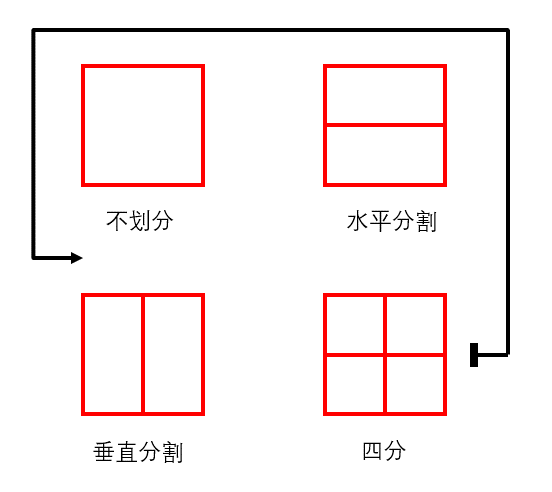
\includegraphics[width = 0.4\textwidth]{coding-vp9-mode}
  \caption{VP9的四种划分模式}
  \label{fig:coding-vp9-mode}
\end{figure}

举例来说,假设我们对某一个64x64的块进行划分,过程如下:
\begin{enumerate}
  \item 64x64的块采用四分模式,它的四个32x32的子块按从左到右从上到下的顺序,继续递归划分。
  \item 左上的32x32子块被认为不必继续划分,子块划分停止;而右上的子块则被认为应当采用水平分割模式
  分割为1和2,然后划分停止。
  \item 对左下角的块,它被四分,4个16x16的子块开始新一轮的、更小尺寸的分割,他们有的被垂直分割(例如3和4),
  有的停止分割(例如5和6),也有的被四分后继续递归。这一过程持续到最小的块为4x4时,递归结束。
  \item 右下角的块也被判定为不必再划分,整个64x64块的划分过程结束。
\end{enumerate}

\begin{figure}[H] % use float package if you want it here
  \centering
  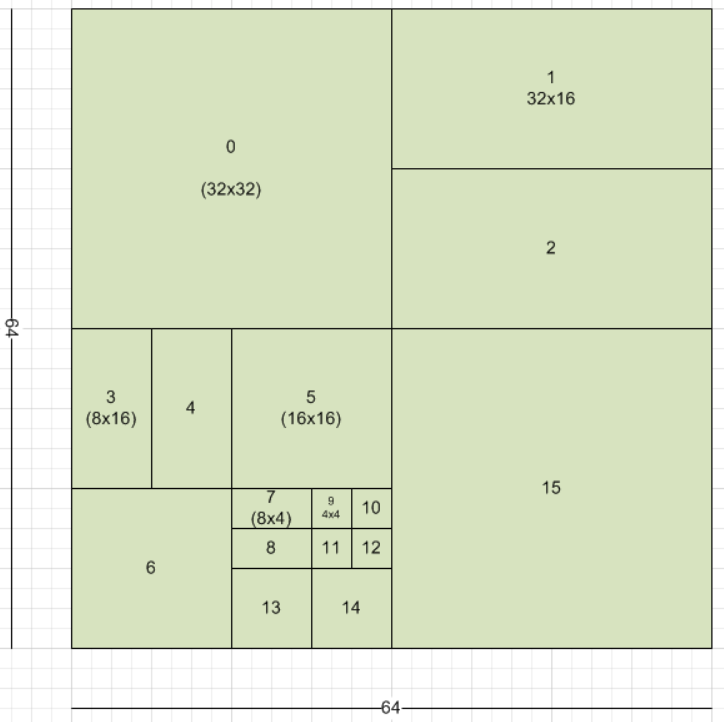
\includegraphics[width = 0.55\textwidth]{coding-vp9-partition-demo}
  \caption{VP9四叉树划分示例}
  \label{fig:coding-vp9-partition-demo}
\end{figure}

在将块划分为四叉树结构的过程中,每一叶子节点将被标记,以便后续的处理。首先是段编号,该编号允许
后续的变换过程中按块使用量化器或是环路滤波;此外,段编号还可用于编码固定的参考块,或是将块标记
为跳过,这一点在处理视频流中的静态背景时是十分有效的。与此同时,有一些叶子节点将被打上跳过标记,
拥有这种标记的块没有残差系数。另外,还需要决定节点的预测模式,分为帧内预测与帧间预测两种,两种预测
模式将在 \ref{subsec:intra}节 和 \ref{subsec:inter}节 中详细介绍。需要明确的是,将块组织为四叉编码树,
很大程度上是为了后续的变换过程。在VP9中,变换的基本单位是4x4、8x8、16x16、32x32的块,对于由水平分割
或是垂直分割产生的非正方形子块,将被分为两个或是多个部分进行变换,即,一个块是可以包含多个变换块的。

\begin{figure}[H]
  \centering%
  \begin{subfigure}{0.43\textwidth}
    \centering
    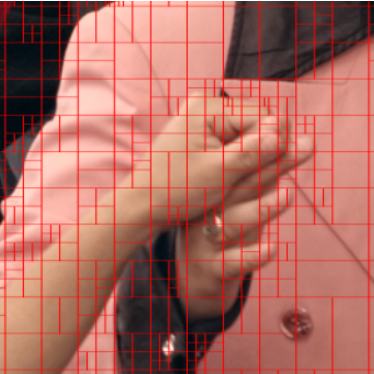
\includegraphics[height = 4.5cm]{coding-block-partition}
    \caption{块的四叉树划分}
  \end{subfigure}%
  \hspace{2em}%
  \begin{subfigure}{0.43\textwidth}
    \centering
    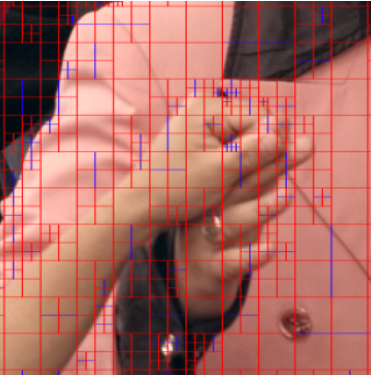
\includegraphics[height = 4.5cm]{coding-transform-partition}
    \caption{变换单元的划分}
  \end{subfigure}
  \caption{块与变换单元组织示意}
\end{figure}

\subsection{帧间预测}
\label{subsec:inter}

当一些块完成编码后,就可以作为后续块编码的参考使用。当一个块决定使用帧间预测模式时,它通常会去寻找
与它相近的1到2个已编码的块来作为参考,该块与用来参考的块两者间的向量被称为运动矢量。之所以会去寻找
参考块,是基于视频流的画面通常是连续的、不会发生体突变的这样一个事实,因此,在相邻的两帧中,我们可以
期望在块级别上会有相当多的块是非常相似的。当使用2个参考块时,我们采用两个参考块预测值的平均值来作为当前
块最终的预测值。并且在VP9中,参考块以 $1/8$ 像素为步长进行移动,由此尽可能保证当前块能找到相似度
尽可能高的参考块,在运动补偿中,将用插值的方式对不足1的亚像素点进行生成。

VP9编码标准中,一个包含8个参考帧的缓存序列会被动态地维护,每当有一帧需要被编码时,序列中的3个可参考帧
会被选取,作为该帧的参考列表,这3个可参考帧中会分别进行运动矢量的搜索,再选出最优的。对于每个
运动矢量的编码,其具有四种模式:NEARESTMV、NEARMV、ZEROMV和NEWMV。ZEROMV表明该块没有移动,具有为零
的运动矢量。除ZEROMV模式外的其余模式中,参考运动矢量列表根据附近块和先前帧中的该块生成,
并做排序。当模式为NEARESTMV或NEARMV时,该块将使用来参考运动矢量列表的第一个或第二运动矢量。如果模式为NEWMV,
则该块将使用全新的运动矢量,将全新运动矢量与NEARESTMV模式中的差值送至运动矢量列表的第一个位置,
与NEARESTMV模式中的运动矢量相加生成新运动矢量。

\begin{figure}[H] % use float package if you want it here
  \centering
  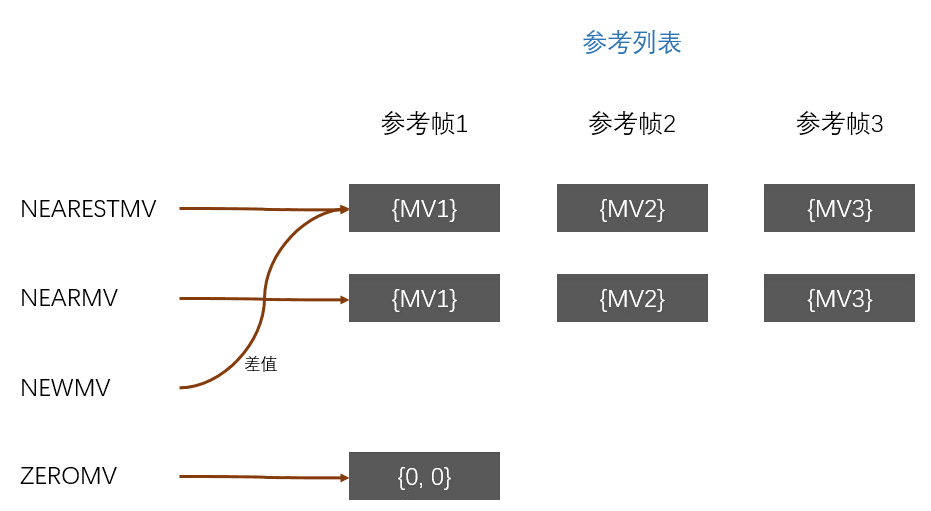
\includegraphics[width = 0.9\textwidth]{coding-ref-list}
  \caption{运动矢量参考列表}
  \label{fig:coding-ref-list}
\end{figure}

\subsection{帧内预测}
\label{subsec:intra}

当帧间预测无法给出令人满意的参考块时,帧内预测也是一种可以考虑的预测模式。当前块的左、左上、上、右上等方向的
相邻像素点可以做为参考,用于预测。VP9制定了总共10种帧内预测方式,其中有8种是按方向预测,另外为TM模式和DC模式。

按方向预测是指VP9中规定了8种方向,根据当前块的具体情况,选择一个合适的方向,从该方向上的已编码的块中,寻找在
边缘相邻的像素点,并以此预测当前块中对应像素点的值。

\begin{figure}[H]
  \centering%
  \begin{subfigure}{0.43\textwidth}
    \centering
    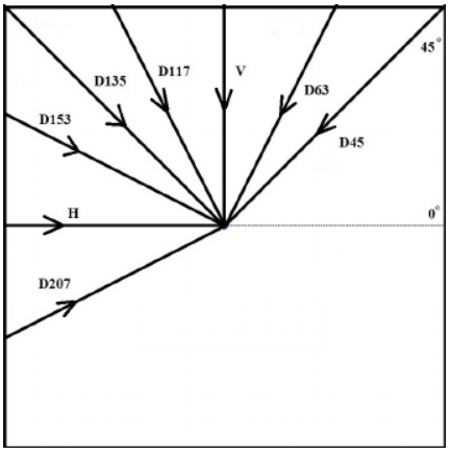
\includegraphics[height = 4.5cm]{coding-intra-direction}
    \caption{VP9帧内8种定向预测}
  \end{subfigure}%
  \hspace{2em}%
  \begin{subfigure}{0.43\textwidth}
    \centering
    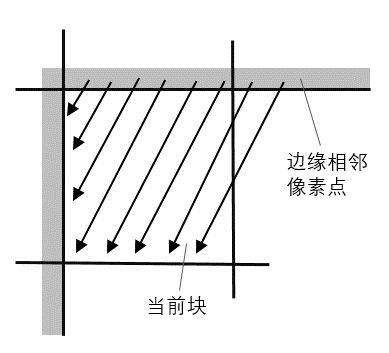
\includegraphics[height = 4.5cm]{coding-intra-direction-demo}
    \caption{以63度为方向进行预测}
  \end{subfigure}
  \caption{按方向预测模式与示例}
\end{figure}

% TM为True-Motion的缩写,该模式使用当前块的左上方已编码相邻块的3个像素点,对当前像素点的值使用 公式~\ref{eq-coding-tm} 进行预测。

% \begin{equation}
% \label{eq-coding-tm}
% p(x, y) = L_x + T_y -TL
% \end{equation}

% 这里,$p(x, y)$为当前待预测像素点的预测值,$L_x$为当前像素点左侧已编码块中的相邻像素点,$T_y$为当前像素点上方已编码块
% 中的相邻像素点,$TL$则是左上角块中的相邻像素点。 图~\ref{fig:coding-intra-tm} 给出了简单示意图,浅色部分示意了一个
% 4x4的当前块,灰色部分标识了位于左上方向的9个已编码块中的像素点,这些像素点被用来预测当前块中的各个像素点。一般地,
% 对于一个$N x N$的块,TM模式使用左上方的$2N+1$个相邻已编码像素点,根据 公式~\ref{eq-coding-tm} 给出预测值。

% \begin{figure}[H] % use float package if you want it here
%   \centering
%   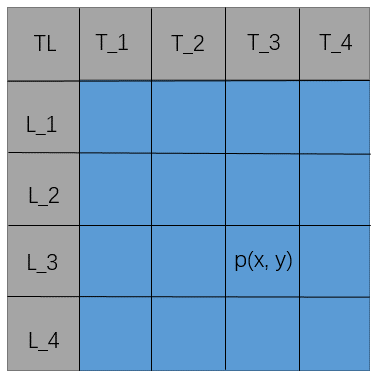
\includegraphics[width = 0.4\textwidth]{coding-intra-tm}
%   \caption{对4x4的块进行帧内预测}
%   \label{fig:coding-intra-tm}
% \end{figure}

% 最后一种DC模式则是Direct-Current,该模式使用均值对整个块中的像素点进行预测,如 \ref{eq-coding-dc} 所示。

% \begin{equation}
% \label{eq-coding-dc}
% p(x, y) = \frac{1}{2N} (\sum_{i=1}^N T_i + \sum_{i=1}^N L_i)
% \end{equation}

% 这里,不妨认为当前块是一个大小为$NxN$的块,DC模式将左和上的$2N$个相邻已编码像素点的值做平均,将该平均值作为块内每
% 个点的预测值。

\subsection{残差编码}

首先给出DCT和ADST两种变换的数学公式(一维情形),如 公式~\ref{eq-coding-dct} 和 公式~\ref{eq-coding-adst} 所示。

\begin{equation}
\label{eq-coding-dct}
X_n = \sum_{n=1}^N x_ncos(\frac{(2n-1)(k-1) \pi}{2N}) \;\; k=0,...,N-1
\end{equation}

\begin{equation}
\label{eq-coding-adst}
X_n = \sum_{n=1}^N x_nsin(\frac{(2n-1)(2k-1) \pi}{4N}) \;\; k=0,...,N-1
\end{equation}

% 介绍DCT和ADST


为便于理解,我们不妨假设我们有原始帧$A$,经过划分为四叉树、帧间预测、帧内预测等一系列过程,我们得到了由预测像素值构成的
帧$\mathop{{A}'}$,则残差为 $A - \mathop{{A}'}$,对该残差矩阵进行变换、编码即可。所谓变换,是指对残差矩阵在水平、垂直
两个维度上,分别使用DCT或是ADST变换,依据预测模式的不同,两个维度上具体使用哪种变换也会不同。
% ,具体规则如下:

% \begin{itemize}
%   \item 对于仅依赖上方相邻像素点的帧内预测模式(帧内按方向预测中的垂直预测模式),水平方向上使用DCT而垂直方向上使用ADST
%   \item 对于仅依赖左侧相邻像素点的帧内预测模式(帧内按方向预测中的水平预测模式),水平方向上使用ADST而垂直方向上使用DCT
%   \item 对两侧相邻像素点都有依赖的帧内预测模式(TM以及按向下或右的方向帧内预测模式),两个方向上都应当使用ADST
%   \item 所有帧间预测、DC以及其他按方向预测,两个方向上都使用DCT
% \end{itemize}

变换后的残差矩阵会经过量化过程,使右下角的部分高频低能量分量被过滤掉,从而减少所需编码的数据量。

\subsection{后续过程}

视频编码的整个过程是较为漫长而复杂的,如 \ref{sec:content}节 所述,对视频编码标准的优化可以针对其中的某一个步骤进行,
考虑到本文主要针对将块进行四叉树划分这个过程,且可能需要结合或是影响到预测以及变换过程,因此对这些部分进行了较为详细
的介绍。后续的编码过程在本文中的重要性相对较低,因此仅作简单的介绍。

在完成残差编码后,变换块和预测块间会出现极不平滑的边缘,为了平滑这些边缘,VP标准使用了环路滤波器。总计4个环路滤波器
在块的边缘独立工作,修改16、8、4或2个像素点以平滑过渡。较小的变换只允许小的滤波器,而最大的变换可以用任意滤波器处理,
具体选取哪个取决于滤波器强度和边缘硬度。

最后,VP9标准使用二进制算术范围编码器,每个符号具有与其相关联的概率表,这些概率既可以是默认值,也可以基于先前帧的解码
数据的熵,在下一帧的编码开始前动态更新,这是一种能使概率有效适应数据熵的方法。

\section{AV1视频编码标准}

\subsection{概述}

如 \ref{sec:background}节 所述,AV1在编码框架上与VP9等现行的编码标准是一致的,且标准的制定上很大程度上以VP9作为基础。
事实上,这一标准原定应为VP10,但2015年底成立的AOM负责其制定后,最终定为AV1。因此,在 \ref{sec:vp9} 已经对VP9的关键
环节做了较为详细的介绍的基础上,对于AV1以对比的形式进行介绍,是十分合理且易于理解的。

接下来几部分依次介绍了AV1与VP9在四叉编码树的划分上、帧间预测、帧内预测等方面的不同。最后,对于其他一些本文不重点讨论的
步骤上两者的差异,也进行了一些简要的介绍。

\subsection{块的划分}

相较于VP9将帧划分为64x64的块,AV1为了适应更高分辨率的视频,采用128x128作为帧的划分尺寸,避免了处理更高分辨率视频
时块数量的爆炸。在块的划分上,AV1仍采用四叉编码树的组织形式。

相较于VP9的4中块划分模式,AV1将其拓展到了如 图~\ref{fig:coding-av1-mode} 所示的多达10种。VP9中的4种传统划分方式得到了
保留,在此基础上,水平划分HORZ和垂直划分VERT又拓展出了新型的“T”型分割:在HORZ的基础上,将上方的子块再次分割所得到
的变种分割方式被称为HORZ\_A;而将下方子块再次分割的变种则称为HORZ\_B;同理VERT也有两种被称为VERT\_A和VERT\_B的变种。
此外,水平四等分HORZ\_4和垂直四等分VERT\_4也被加入到了AV1的划分模式中,由此构成了总计多达10种的划分模式。需要注意的
是,仅SPLIT模式生成的子块参与递归式的下一轮划分,HORZ\_A、HORZ\_B、VERT\_A、VERT\_B中的正方形子块并不会再次参与划分。

\begin{figure}[H] % use float package if you want it here
  \centering
  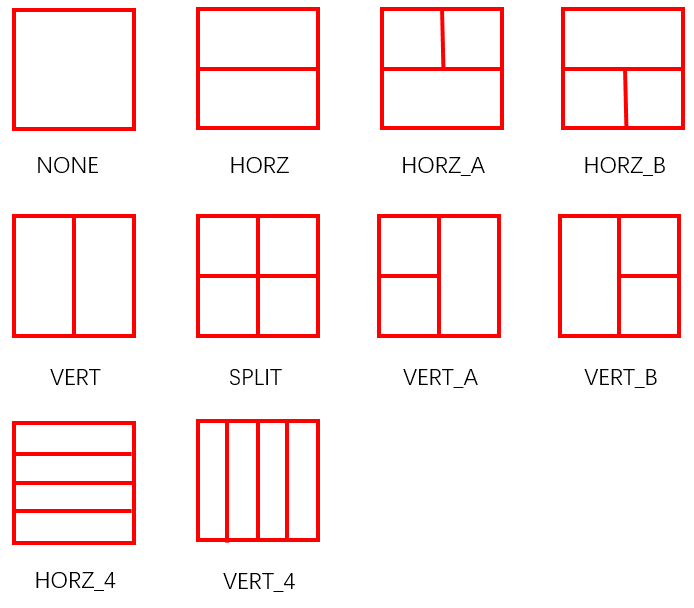
\includegraphics[width = 0.7\textwidth]{coding-av1-mode}
  \caption{AV1中10种块划分方式}
  \label{fig:coding-av1-mode}
\end{figure}

除了划分模式的拓展,在对尺寸较小的子块处理的灵活性上,AV1也进行了改进。VP9对于4x4的子块有着较多的限制,包括需要将参考
块与差值滤波器结合使用、帧内与帧间混合的预测模式在块的尺寸小于8x8时不能使用等。而AV1则放开了部分限制,在色度层上,允许
以2x2的尺寸进行帧间预测,但最小变换单元尺寸仍保持4x4;在亮度层,允许较小尺寸的块使用帧内、帧间混合预测模式,但在色度
层不允许;为了保持硬件吞吐率与VP9一致,AV1仍禁止小于8x8的块使用复合模式(指帧间预测中使用多于一个运动矢量预测的模式)。

% \subsection{帧间预测}
\subsection{帧间、帧内预测}

在帧间预测上,AV1与VP9一样动态地维护一个长度为8的帧缓存序列。不同的是,VP9标准规定从其中选取3帧用于参考,而AV1将这一数字
扩大到了7,即会从缓存序列中选择7帧作为参考。
在运动估计的过程中,VP9会在周围块进行扫描,相邻块的运动向量纳入候选序列中,三个参考列表每个会维护2个运动向量。而AV1标准进行
了拓展,一方面,相邻块的搜索范围有所扩大,使得更多的运动向量有机会进入参考运动向量列表;另一方面,在每个参考列表中,AV1
会维护四个参考运动向量,且不同于VP9中参考列表中向量的排名与搜索顺序有较强的相关性,AV1使用概率模型对参考运动向量做排序,
使得靠前的结果有着更高的可信度。

\begin{figure}[H] % use float package if you want it here
  \centering
  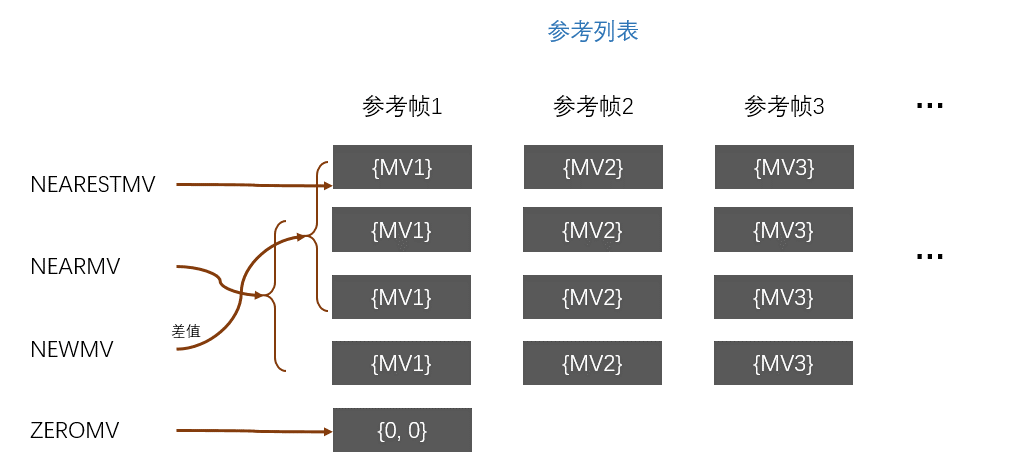
\includegraphics[width = 0.9\textwidth]{coding-av1-ref-list}
  \caption{AV1运动矢量参考列表}
  \label{fig:coding-av1-ref-list}
\end{figure}

在复合模式上,VP9仅支持两运动向量以$1/2$、$1/2$为比例进行复合,且这两个运动向量不能是同侧的。AV1中放开了对同侧的限制,
即其允许两同侧的运动向量复合使用,进行预测;此外,AV1中的复合更为广义,不再局限于两种帧间预测器复合,帧间-帧内的复合
也是可行的。

\begin{figure}[H] % use float package if you want it here
  \centering
  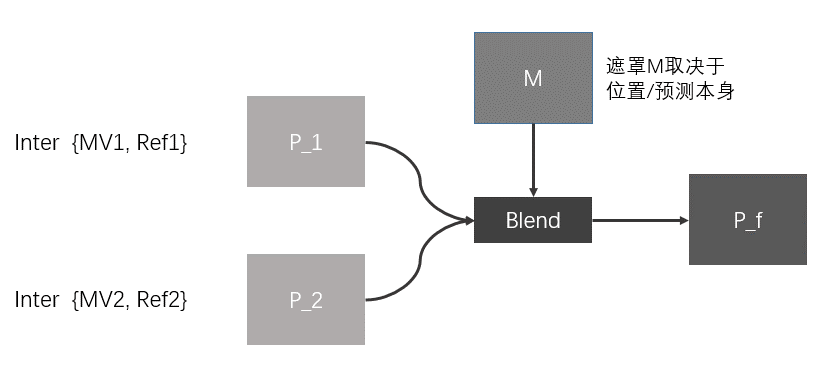
\includegraphics[width = 0.8\textwidth]{coding-av1-inter-inter}
  \caption{帧间-帧间复合模式}
\end{figure}

\begin{figure}[H] % use float package if you want it here
  \centering
  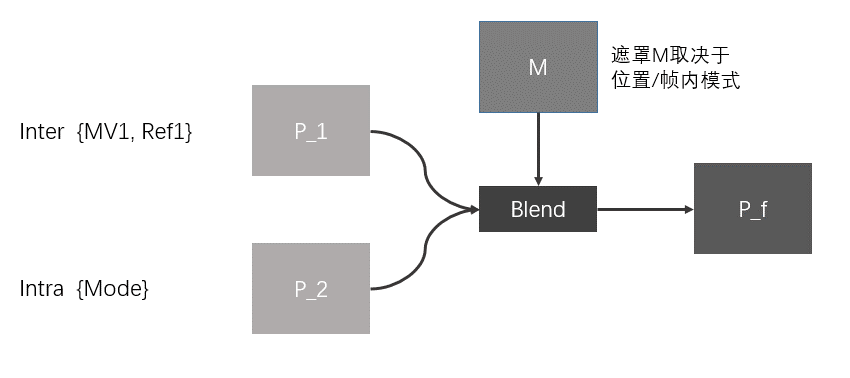
\includegraphics[width = 0.8\textwidth]{coding-av1-inter-intra}
  \caption{帧间-帧内复合模式}
\end{figure}

在帧内预测上,VP9中的8种按方向预测的模式得到了保留,并且根据块的尺寸的不同,所能使用的预测方向被拓展到了56个。根据不同
的块的尺寸选择更加细致的预测方向,对于预测结果的准确性是有着积极意义的。而非按方向预测中的TM模式被Paeth所取代,DC模式
得到了保留,额外新加入的还有调色板模式(Palette Mode)等。


% \subsection{帧内预测}

% 在帧内预测上,VP9中的8种按方向预测的模式得到了保留,并且根据块的尺寸的不同,所能使用的预测方向被拓展到了56个。根据不同
% 的块的尺寸选择更加细致的预测方向,对于预测结果的准确性是有着积极意义的。而非按方向预测中的TM模式被Paeth所取代,仍以
% 图~\ref{fig:coding-intra-tm} 为例,Paeth模式将根据公式 \ref{eq-coding-paeth} 给出预测值。

% \begin{equation}
% \label{eq-coding-paeth}
% P_{Paeth}(x, y) = argmin|x-P_{TM}(x,y)|, \; x \in \{L_x,T_y,TL\}
% \end{equation}

% 这里,$P_{Paeth}(x, y)$ 为Paeth模式给出的预测值,他由$P_{TM}(x,y)$(TM模式给出的预测值)与$T_y$、 $L_x$、$TL$三个
% 候选点差的绝对值中的最小者决定。这一方法会选择梯度最小的方向作为预测的方向,以计算量有所增加为代价,能给出比TM模式更好的
% 预测结果。

% 此外,非固定方向的预测方法中还加入了平滑模式,该模式分为水平、垂直、双边三种子模式。该模式加入平滑因子函数$w(x)$,根据
% 像素点在块中位置的不同使用不同的平滑因子,将候选点的值做线性加权来给出预测值。需要说明的是,\ref{fig:coding-smooth-function}
% 给出的仅为趋势示意图,实际实现时,$w(x)$是离散的,根据块的大小预先设定了一系列的离散值供预测函数使用。在水平平滑模式中,
% 选取左侧和右上角的像素点,并选用像素点在水平方向的距离计算平滑因子;垂直平滑模式则选取上方和左下角的像素点,并选用垂直
% 方向的距离生成平滑因子;双边模式则结合上述两种模式给出的预测值做平均,作为最终的结果。 \ref{eq-coding-smooth-mode}
% 给出了公式化的描述,$P_{SMOOTH\_H}$、$P_{SMOOTH\_V}$、$P_{SMOOTH\_B}$依次为水平、垂直、双边平滑模式。

% \begin{equation}
% \label{eq-coding-smooth-mode}
% \begin{split}
% P_{SMOOTH\_H} & = w(x)L + (1-w(x))TR \\
% P_{SMOOTH\_V} & = w(y)T + (1-w(y))BL \\
% P_{SMOOTH\_B} & = \frac12(P_{SMOOTH\_H} + P_{SMOOTH\_V})
% \end{split}
% \end{equation}

% \begin{figure}[H]
%   \centering%
%   \begin{subfigure}{0.43\textwidth}
%     \centering
%     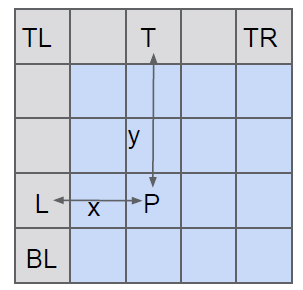
\includegraphics[height = 4.5cm]{coding-smooth-mode}
%     \caption{平滑模式预测示意图}
%   \end{subfigure}%
%   \hspace{2em}%
%   \begin{subfigure}{0.43\textwidth}
%     \centering
%     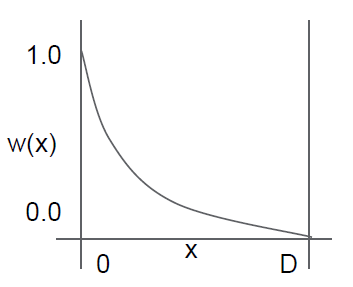
\includegraphics[height = 4.5cm]{coding-smooth-function}
%     \caption{平滑因子函数$w(x)$}
%     \label{fig:coding-smooth-function}
%   \end{subfigure}
%   \caption{帧内预测平滑模式}
% \end{figure}

% % 展开?
% 此外,VP9中的DC模式得到了保留,额外新加入的还有调色板模式(Palette Mode)等。

\subsection{其他}

在对残差矩阵的变换、编码上,VP9 依据预测方式的不同,从 $\{DCT, ADST\}^2$ 选择二维变换对残差矩阵进行处理。在AV1中,
仍是分水平、垂直两个方向分别作一维变换,不同的是,除DCT和ADST外,还加入了ADST的逆变换(Flip ADST)以及恒等变换(IDTX),
由此将变换的可能性拓展到了 $|\{DCT, ADST, FlipADST, IDTX\}^2|$ 总计16种。此外,不同于VP9仅支持正方形的块作为变换的
基本单位,AV1对一些尺寸的矩形块作为变换的基本单位有了支持。

% 其他?